\chapter{Metodología de la Investigación}
\section{Diseño de la investigación}
En esta sección se detallan el diseño, tipo y enfoque de la investigación, así como la población y la muestra.

\subsection{Tipo de investigación}
Se ha identificado que este estudio posee un diseño experimental con el propósito de establecer el tipo de investigación. Como lo dice \cite{bk_hernandez2014metodologia}, en la obra titulada \citetitle{bk_hernandez2014metodologia}, busca determinar la consecuencia de una razón manipulada. Específicamente, se clasifica como un diseño experimental puro debido a la utilización intencionada de variables independientes (modificadas, eliminadas o añadidas) para evaluar su influencia en la variable dependiente, que en este caso es la segmentación avanzada de características morfológicas faciales (arrugas y manchas) en imágenes de rostros faciales.

% \subsection{Alcance de la investigación}
% El alcance de esta investigación se enfoca exclusivamente en la segmentación de arrugas, poros y manchas en imágenes faciales en dos dimensiones (2D). Este trabajo está orientado al sector cosmético y de belleza, en lugar de la dermatología médica, y no abordará el diagnóstico de otras condiciones cutáneas. Las imágenes provendrán de bases de datos públicas y se seleccionarán muestras representativas de diferentes tipos de piel y regiones geográficas para asegurar diversidad en los datos. La temporalidad del estudio abarca un período de aproximadamente 6 a 12 meses, desde la recolección de datos hasta la validación del modelo \cite{statista2023, aad2022}.

\subsection{Enfoque de la investigación}
Este estudio adoptó un enfoque cuantitativo, conforme a lo explicado por \cite{bk_hernandez2014metodologia} en su libro \citetitle{bk_hernandez2014metodologia}. Este enfoque se basa en la recopilación de datos para comprobar hipótesis mediante mediciones numéricas y análisis estadísticos, con el objetivo de identificar patrones de comportamiento y validar teorías. La metodología empleada sigue los diez pasos del proceso cuantitativo descritos por el autor, aplicados desde la formulación de la idea hasta la presentación de los resultados finales en el informe de investigación, ya que se busca desarrollar un sistema de segmentación para detectar características morfológicas de la piel facial mediante redes neuronales convolucionales (CNN) y analizar su efectividad con métricas cuantitativas, como precisión, recall, F1-score y AUC-ROC. Este enfoque permitirá evaluar el desempeño del sistema en la detección de arrugas, poros y manchas, proporcionando resultados medibles y objetivos. \parencite{esteva2017} Al emplear técnicas de aprendizaje profundo, el estudio pretende optimizar la precisión en la segmentación de características faciales, aplicando un marco metodológico replicable y sistemático. \parencite{phillips2020}

\subsection{Población}
La población de este estudio se compone de imágenes faciales representativas de personas con diversas edades, géneros y tipos de piel. Específicamente, estas imágenes muestran características morfológicas que se asocian con arrugas y manchas faciales. Debido a la orientación del enfoque en el problemas estéticos, la población abarcaba imágenes de piel con claras imperfecciones y piel sin e incidencias asignadas. Así, el alcance de la población se determina como diverso y completo, asegurando la inclusión de imágenes que representa una amplia gama de condiciones de la piel. Finalmente, resulta esencial agregar diversidad geográfica, ya que ciertas diferencias geográficas.
\subsection{Muestra}
La muestra de la investigación comprenderá una parte de aproximadamente 5000 retratos faciales. Estas imágenes se seleccionarán mediante muestreo basado en estratos, lo que garantizará una representación uniforme en diferentes categorías de edad, identidades masculinas y femeninas y pigmentación dérmica variable La lista también tendrá imágenes con diferentes tamaños y claridad, mostrando varios tipos de arrugas y manchas, asegurándose de que el grupo muestre condiciones reales de la piel Los usaremos para enseñar, verificar y desafiar nuestro modelo de segmentación avanzada, asegurándonos de que funcione bien en la vida real con mucha variedad.

\subsection{Operacionalización de Variables}
Los detalles acerca de cómo se definen y miden las variables de estudio se presentan en la Tabla \ref{tabla:variables}.
%\begin{table}[h!]

\begin{longtable}{>{\raggedright\arraybackslash}m{3cm} >{\raggedright\arraybackslash}m{2cm} >{\raggedright\arraybackslash}m{2cm} >{\raggedright\arraybackslash}m{3cm} >{\raggedright\arraybackslash}m{2cm} >{\raggedright\arraybackslash}m{2.5cm}}
    \caption{Matriz de Variables Principales.}
    \label{tabla:variables}\\
    \hline
    VARIABLE & DIMENSIÓN & INDICADOR & DEFINICIÓN DEL INDICADOR & TÉCNICA DE MEDICIÓN & ESCALA \\
    \hline
    Independiente: Imágenes de Rostros Faciales & Calidad de la Imagen & Resolución & Número de píxeles por unidad de área (píxeles por pulgada) & Análisis de propiedades de la imagen & ppi (píxeles por pulgada) \\
    \cline{2-6}
     & Detalle de Rostro Facial & Características Morfológicas Faciales Identificables & Cantidad de Características Morfológicas Faciales (arrugas y manchas) claramente identificables en la imagen & Contaje manual o mediante segmentación de análisis de imágenes & Número \\
    \hline
    Dependiente: Modelo de Segmentación Avanzada de Características Morfológicas Faciales & Precisión & Diferencia de Segmentación del Modelo vs Real & Diferencia entre la Segmentación por el modelo y la real medida & Comparación de resultados de simulación y segmentación real & Valor entre 0 y 1 \\
    \cline{2-6}
     & Índice de Sorensen-Dice & Similitud espacial & Medida de similitud que evalúa el solapamiento entre las áreas segmentadas por el modelo y las reales & Cálculo del índice usando máscaras binarias predicha y real & Valor entre 0 y 1 \\
    \cline{2-6}
     & Coeficiente de Jaccard & Similitud de conjunto & Proporción entre la intersección y la unión de las áreas segmentadas por el modelo y las reales & Cálculo del índice comparando máscaras de salida y verdad de terreno & Valor entre 0 y 1 \\
    \cline{2-6}
	& Entropía Cruzada & Desempeño de clasificación del modelo &  Medida de pérdida entre la distribución de probabilidad predicha y la real en cada píxel segmentado & Evaluación de la función de pérdida durante el entrenamiento del modelo & Escala real positiva \\
    \hline
\end{longtable}
%\par	%%Salto de linea
%\bigskip
\begin{flushleft}	%%Alinear a la izquierda sin justificar
	\small Fuente: Elaboración propia.
\end{flushleft}
%\end{table}

\section{Técnicas de recolección de datos}
La recolección de imágenes de características morfológicas faciales es un paso crucial para la creación del modelo de segmentación avanzada de estas. Una de las técnicas más accesibles y efectivas para obtener estas imágenes es a través del uso de bases de datos públicas como se ve en la Figura \ref{3:fig2}y repositorios en línea. Estas fuentes ofrecen una amplia variedad de imágenes de rostros faciales, que pueden ser utilizados para modelar y crear el modelo de segmentación avanzada.

\begin{figure}[h]
	\begin{center}
		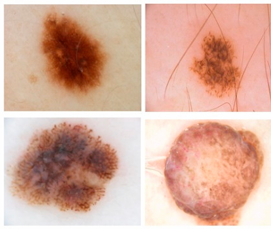
\includegraphics[width=0.75\textwidth]{3/figures/datapaper.png}
		\caption[Dataset usado en el artículo de \cite{moon2024dermatology}]{Dataset usado en el artículo de \cite{moon2024dermatology}.\\
		Fuente: \cite{moon2024dermatology}. \citetitle{moon2024dermatology}. (p. 4)}
		\label{3:fig2}
	\end{center}
\end{figure}

\begin{itemize}
    \item \textbf{Repositorios de Datasets de Imágenes Faciales}: Existen múltiples repositorios en línea dedicados específicamente a la recopilación y distribución de imágenes faciales. Plataformas como Kaggle, Papers with Code, y OpenML ofrecen conjuntos de datos etiquetados que incluyen rostros humanos con diferentes características morfológicas como arrugas, manchas, expresiones y edades. Estos datasets son fundamentales para el entrenamiento y evaluación de modelos de redes neuronales convolucionales, y suelen estar acompañados de documentación sobre su uso y licencia.
	\item \textbf{Bibliotecas Digitales y Bases de Datos Académicas}: Las bibliotecas digitales y bases de datos académicas también representan una fuente valiosa para obtener datasets faciales. En publicaciones académicas y tesis disponibles en plataformas como IEEE Xplore, SpringerLink, ScienceDirect y Google Scholar, es común encontrar referencias a datasets faciales utilizados en investigaciones previas. Estas fuentes permiten identificar conjuntos de datos validados por la comunidad científica y conocer sus aplicaciones en diferentes contextos, como el reconocimiento facial o el análisis de envejecimiento.
	\item \textbf{Plataformas de Código Abierto y Comunidades de Investigación}: Plataformas como GitHub, Hugging Face y Zenodo son ampliamente utilizadas por la comunidad investigadora para compartir datasets y modelos preentrenados. En estos repositorios, los investigadores publican conjuntos de imágenes faciales junto con scripts de preprocesamiento, anotaciones y arquitecturas de redes neuronales. Muchos de estos recursos se distribuyen bajo licencias abiertas (como CC BY o MIT).
  \end{itemize}


  %\newpage
\section{Técnicas para el procesamiento y análisis de la información}

\subsection{Metodología de implementación de la solución}

La creación de un Modelo de Segmentación Avanzada de Características Morfológicas varias fases de desarrollo, que van desde la recopilación de imágenes hasta su despliegue, como se menciona en el trabajo de \cite{yoon2023}. La imagen adquirida debe pasar por un proceso detallado posteriormente para alcanzar su etapa final. La metodología de esta investigación se muestra en la Figura \ref{3:fig3}.

\begin{figure}[h]
	\begin{center}
		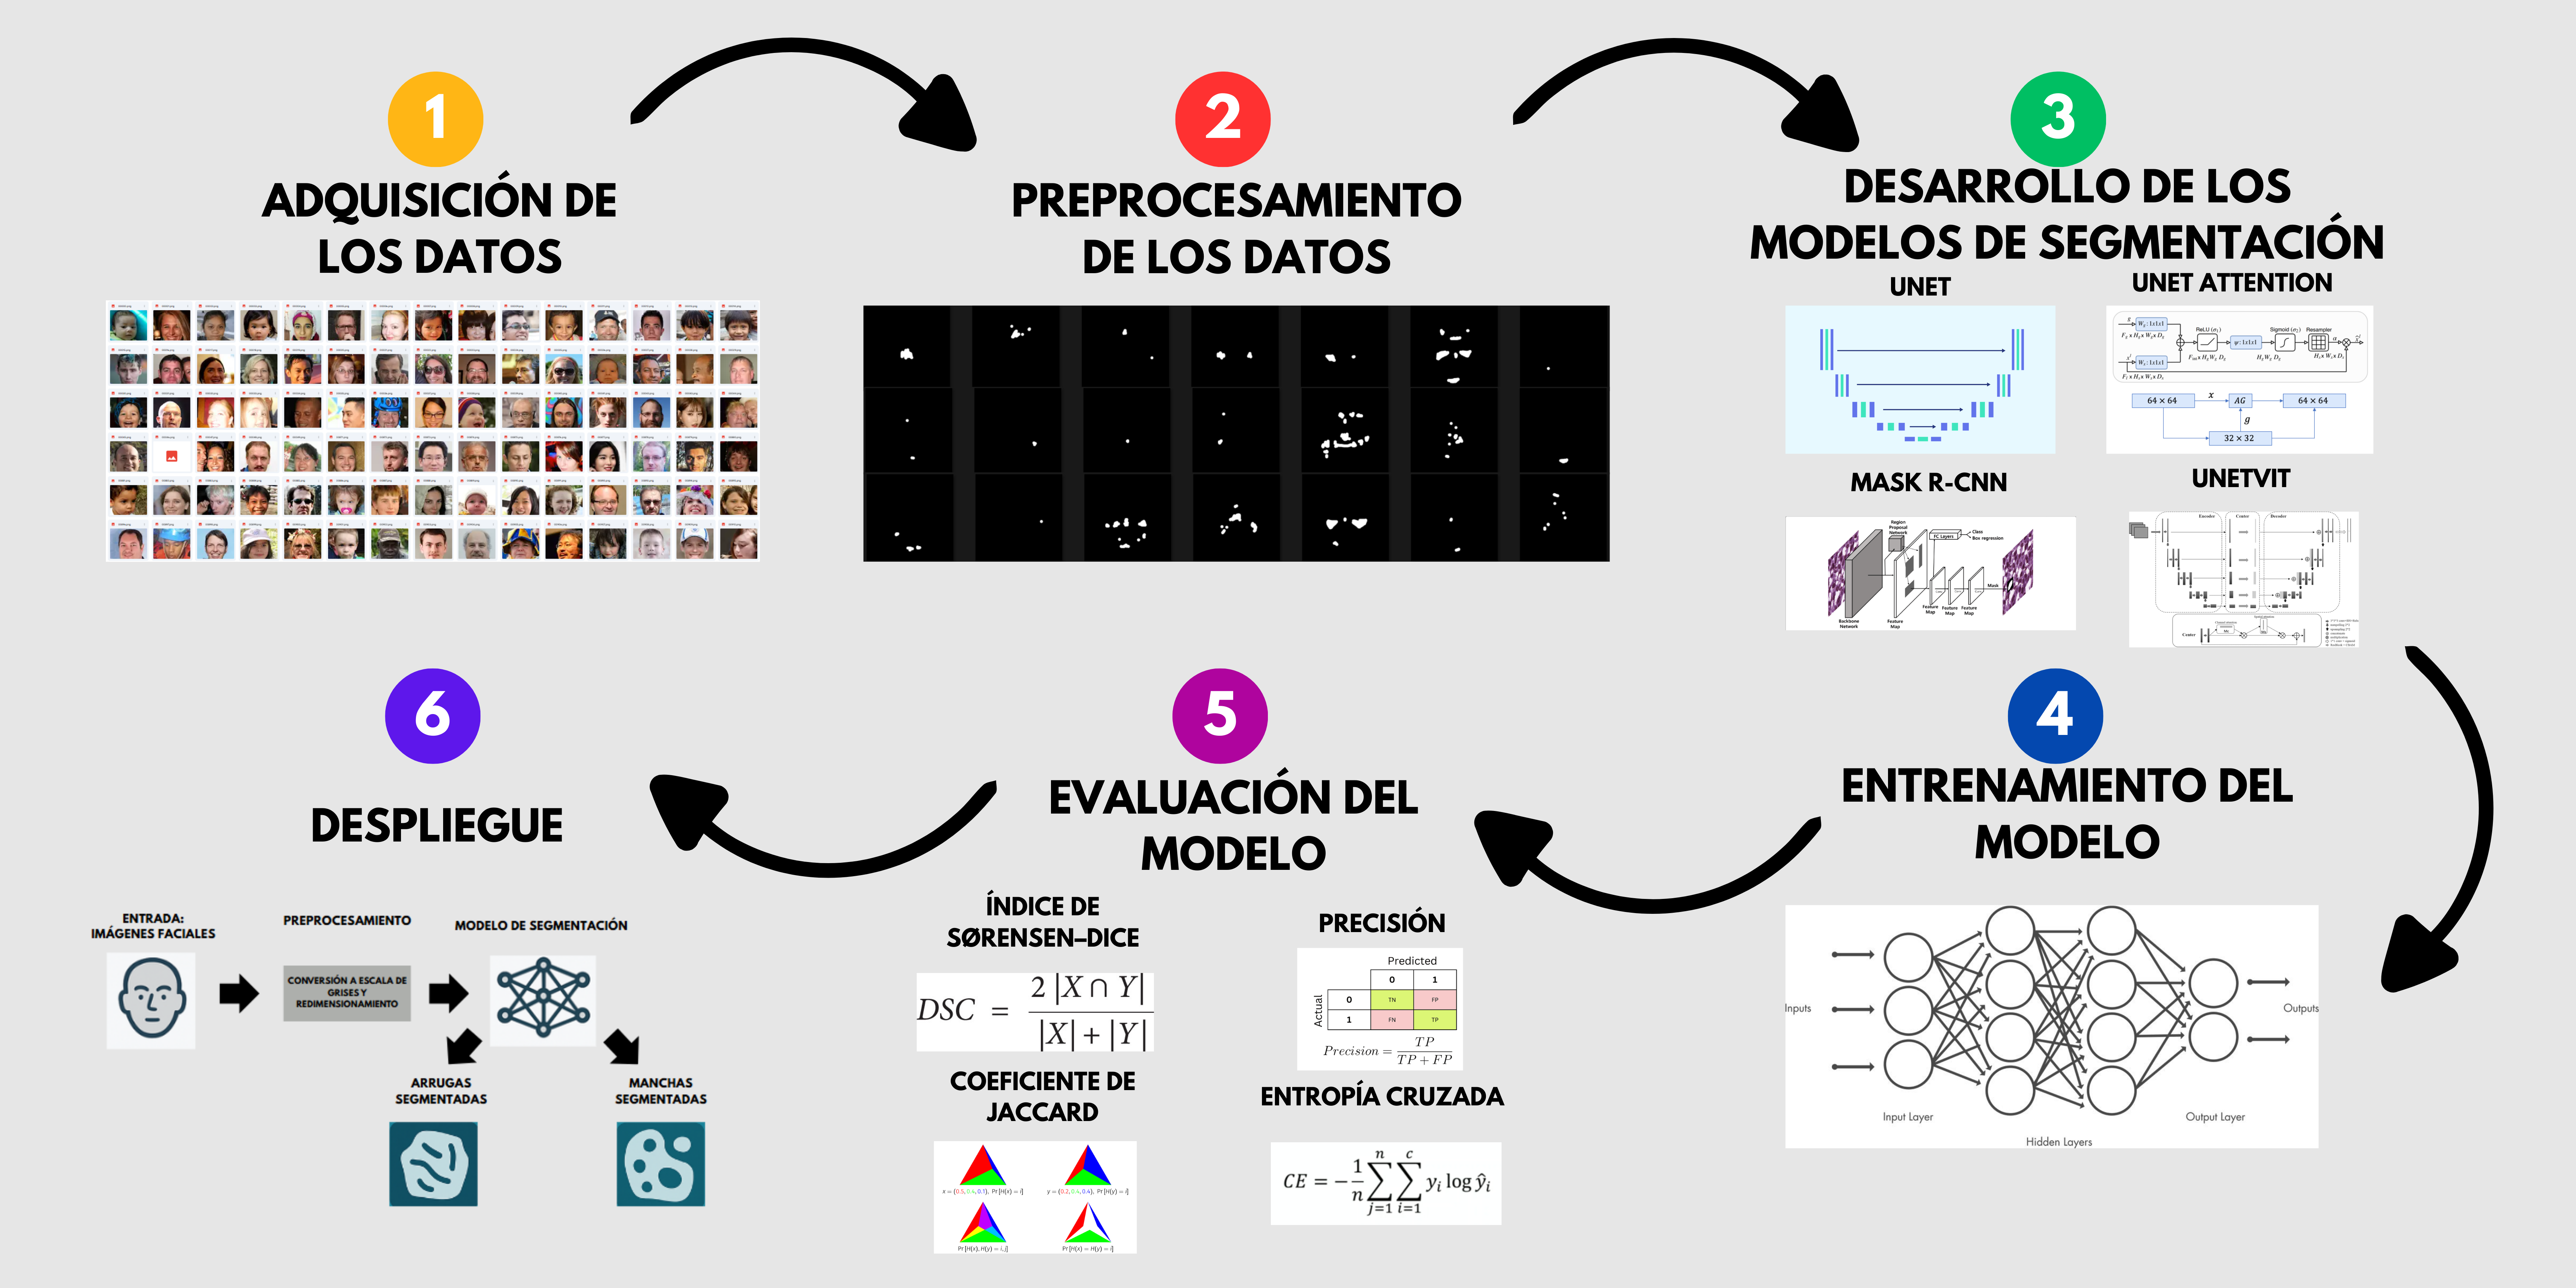
\includegraphics[width=1\textwidth]{3/figures/metodologia.png}
		\caption[Método de Investigación]{Método de Investigación.\\
			Fuente: Elaboración propia.}
		\label{3:fig3}
	\end{center}
\end{figure}


\subsection{Adquisición y Preparación de los Datos}
Se recopilará un conjunto de datos compuesto por imágenes faciales provenientes de bases de datos públicas y privadas. Se priorizarán imágenes que reflejen diversidad en tipos de piel, condiciones morfológicas (como arrugas, poros dilatados y manchas) y niveles de calidad visual. Cada imagen será etiquetada manualmente para clasificar las características específicas en categorías relevantes, como "arrugas incipientes", "poros dilatados" o "manchas hiperpigmentadas".

Durante esta etapa, se planea realizar las siguientes acciones:
\begin{itemize}
    \item \textbf{Exploración inicial:} Se analizará el conjunto de datos para identificar inconsistencias, como imágenes corruptas, valores faltantes o clases desbalanceadas.
    \item \textbf{Limpieza:} Se eliminarán imágenes no útiles (mal etiquetadas o de baja resolución) y se corregirán anomalías en las etiquetas.
    \item \textbf{Aumento de Datos:} Se aplicarán técnicas como rotación, escalado, cambios de iluminación y adición de ruido para abordar problemas de desbalanceo y mejorar la capacidad de generalización de los modelos.
    \item \textbf{Preprocesamiento:} Las imágenes se redimensionarán a una resolución uniforme, se normalizarán los valores de color y se convertirán a un formato estándar que facilite su uso en redes neuronales convolucionales.
\end{itemize}

\subsection{Desarrollo de los Modelos de Segmentación}
Se desarrollarán modelos de segmentación de características morfológicas de la piel utilizando Redes Neuronales Convolucionales (CNN), dada su eficacia comprobada en tareas de análisis de imágenes. Las arquitecturas que se implementarán incluyen:

\begin{itemize}
    \item \textbf{U-Net:} Se utilizará por su capacidad para realizar segmentaciones precisas en áreas específicas, como arrugas y poros, gracias a su diseño simétrico que facilita la reconstrucción de imágenes segmentadas \cite{ronneberger2015}.
    \item \textbf{ResNet:} Se probará para capturar características profundas y complejas mediante su estructura de aprendizaje residual, mejorando el rendimiento en imágenes con texturas complejas \cite{he2016}.
    \item \textbf{Modelos híbridos con Vision Transformer (ViT):} Se explorará su uso para la segmentación de patrones más sutiles, aprovechando su enfoque basado en atención combinado con la extracción de características de las CNN \cite{dosovitskiy2020}.
\end{itemize}

El entrenamiento de los modelos se realizará aplicando las siguientes técnicas:
\begin{itemize}
    \item \textbf{Optimización con Adam:} Para garantizar convergencia rápida y eficiente.
    \item \textbf{Data augmentation:} Se emplearán técnicas de aumento de datos para mejorar la robustez del modelo ante variaciones en el conjunto de datos.
    \item \textbf{Validación cruzada:} El conjunto de datos se dividirá en pliegues para evaluar el desempeño del modelo en diferentes particiones.
\end{itemize}

\subsection{Evaluación y Validación del Sistema}
El desempeño del sistema de segmentación será evaluado utilizando métricas específicas para problemas de clasificación y segmentación:
\begin{itemize}
    \item \textbf{Precisión (Accuracy):} Proporción de predicciones correctas sobre el total de predicciones.
    \item \textbf{Recall (Sensibilidad):} Proporción de características positivas correctamente identificadas.
    \item \textbf{F1-Score:} Promedio armónico de precisión y recall, útil para conjuntos de datos desbalanceados.
    \item \textbf{AUC-ROC:} Área bajo la curva ROC para medir la capacidad del modelo de distinguir entre clases.
\end{itemize}

Adicionalmente, se utilizará una matriz de confusión para analizar en detalle los errores cometidos por los modelos, lo que permitirá identificar patrones en los casos mal clasificados.

\subsection{Implementación y Pruebas Finales}
El modelo seleccionado será integrado en un prototipo funcional que permitirá procesar imágenes faciales y generar un reporte detallado de las características segmentadas. Este prototipo incluirá una interfaz amigable que mostrará:
\begin{itemize}
    \item Mapas de calor que destacarán áreas con arrugas, poros dilatados y manchas.
    \item Gráficos comparativos que mostrarán la evolución de las características morfológicas.
    \item Recomendaciones personalizadas basadas en el análisis segmentado.
\end{itemize}

Las pruebas finales se realizarán en un entorno simulado para verificar su rendimiento en casos prácticos, como evaluaciones estéticas en clínicas dermatológicas o la personalización de tratamientos cosméticos.

\section{Metodología para la Medición de Resultados de la Implementación}

Para garantizar la correcta evaluación del sistema, se emplearán las siguientes métricas basadas en la matriz de confusión:
\begin{itemize}
    \item \textbf{Precisión (Accuracy):} \[ accuracy = \frac{TP + TN}{TP + TN + FP + FN} \]
    \item \textbf{Recall:} \[ recall = \frac{TP}{TP + FN} \]
    \item \textbf{Precisión Positiva:} \[ precision = \frac{TP}{TP + FP} \]
    \item \textbf{F1-Score:} \[ F1 = 2 \cdot \frac{precision \cdot recall}{precision + recall} \]
\end{itemize}

Cada métrica será calculada para determinar la efectividad del modelo en la segmentación de arrugas, poros y manchas, evaluando su capacidad de proporcionar predicciones precisas y consistentes en datos no vistos.
%%%%%%%%%%%%%%%%%%%%%%%%%%%%%%%%%%%%%%

\begin{landscape}
	\section{Cronograma de actividades y presupuesto}
	Se propuso un cronograma para la investigación. Conforma desde el inicio hasta ser terminada con la sustentación final planeada para mediados del año 2024. Este se presneta en la Figura \ref{3:fig303}.

	\begin{figure}[!ht]
		\begin{center}
			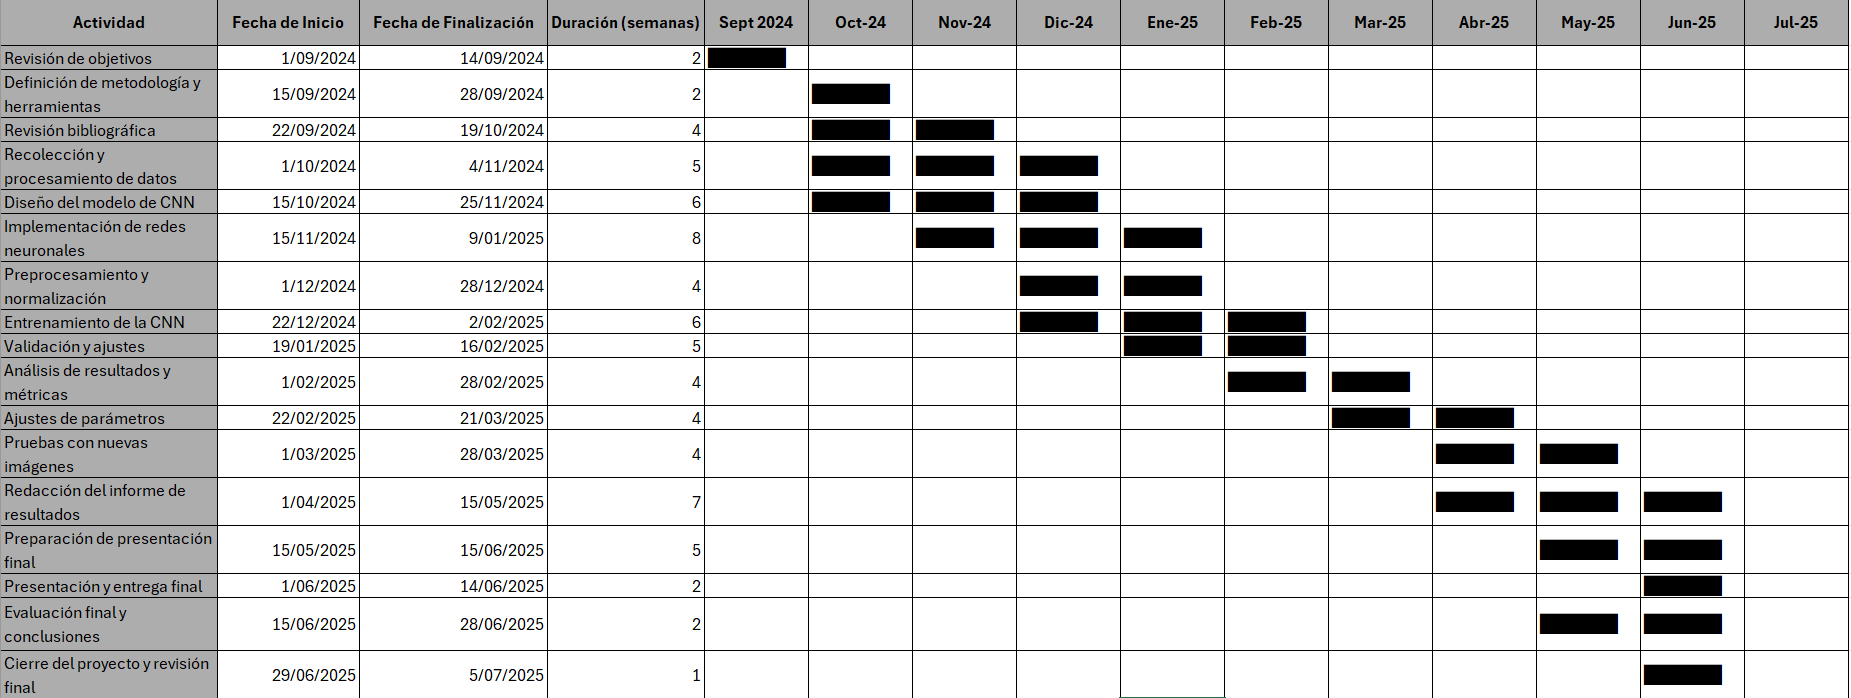
\includegraphics[width=1.50\textwidth]{3/figures/gant.png}
			\caption[Cronograma de actividades]{Cronograma de actividades.\\
				Fuente: Elaboración propia.}
			\label{3:fig303}
		\end{center}
	\end{figure}
	
\end{landscape}
%%%%%%%%%%%%%%%%%%%%%%%%%%%%%%%%%%%%%%%%

%%%%%%%%%%%%%%%%%%%%%%%%%%%%%%%




Se determinó el siguiente presupuesto necesario para la elaboración completa de la investigación. Este se presenta en la Tabla \ref{3:table1}.

\begin{table}[H]
	\caption[Presupuesto]{Presupuesto estimado para el desarrollo del sistema de segmentación morfológica.}
	\label{3:table1}
	\centering
	\small
	\begin{tabular}{llll}
		\specialrule{.1em}{.05em}{.05em}
		{Grupo} & {Item} & {Costo (soles)} & {Subtotal} \\ 
		\specialrule{.1em}{.05em}{.05em}
		\multirow{3}{4cm}{Recursos materiales} 
		& {Laptop de alto rendimiento} & {S/ 7,500.00} & {} \\ 
		& {Materiales de escritorio} & {S/ 150.00} & {} \\
		& {Dispositivo de almacenamiento externo} & {S/ 300.00} & {S/ 7,950.00} \\ 
		\cline{1-4}
		\multirow{3}{4cm}{Software y servicios} 
		& {Licencia de software (Python/IDE)} & {S/ 50.00} & {} \\
		& {Renta de servidor en la nube} & {S/ 500.00} & {} \\
		& {Acceso a bases de datos de imágenes} & {S/ 300.00} & {S/ 850.00} \\ 
		\cline{1-4}
		\multirow{3}{4cm}{Costos académicos} 
		& {Matrícula en Trabajo de Tesis II} & {S/ 375.00} & {} \\
		& {Cuotas de Trabajo de Tesis II} & {S/ 1,044.00} & {S/ 1,419.00} \\ 
		\cline{1-4}
		\multirow{2}{4cm}{Extras} 
		& {Consultorías especializadas} & {S/ 200.00} & {} \\
		& {Movilidad y transporte} & {S/ 300.00} & {S/ 500.00} \\ 
		\specialrule{.1em}{.05em}{.05em} 
		{} & {Total} & {} & {S/ 10,719.00} \\ 
		\specialrule{.1em}{.05em}{.05em}
	\end{tabular}
	\begin{flushleft}	
		\small Fuente: Elaboración propia.
	\end{flushleft}
\end{table}




